\documentclass[../../main.tex]{subfiles}
    
    \lstset{basicstyle=\small,
      showstringspaces=false,
      commentstyle=\color{black},
      keywordstyle=\color{blue}
    }

    \graphicspath{{images/Vision/}{../../images/Vision/}}

    \begin{document}
    \subsection{Vision}
    Im Kapitel Objekterkennung basieren viele Lösungsentscheidungen auf Erkennung mittels Kamera. Hierbei wird die Kamera verwendet um Informationen aufzunehmen. Die Verarbeitung der Informationen und schlussendlich die Objekterkennung erfolgt softwaretechnisch. Abbildung \ref{fig:vision_ablauf} zeigt den prinzipieller Ablauf einer Bildverarbeitung inklusiver Featureerkennung.\\
    \begin{figure}[H] %Ablaufdiagramm Vision
        \centering
        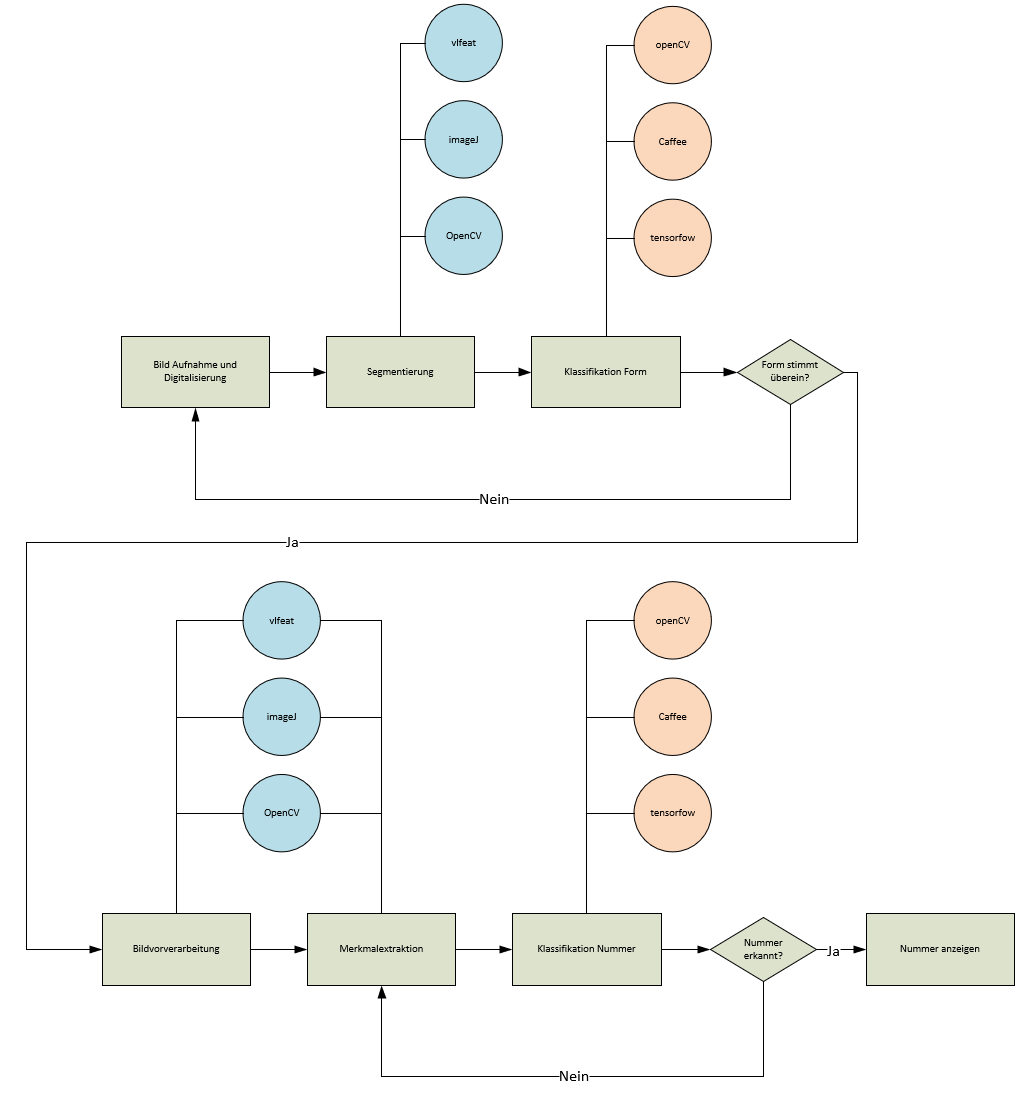
\includegraphics[width=0.8\textwidth]{Ablauf_vision.png}
        \caption{Ablaufdiagram Objekterkennung mittels Software}
        \label{fig:vision_ablauf}
    \end{figure}

    \subsubsection{Bildverarbeitung}
        Wie im Ablaufdiagram \ref{fig:vision_ablauf} ersichtlich, wird die Bildverarbeitung mehrmals angewendet. In der Segmentierung, Bildvorverarbeitung und Merkmalextraktion wird das Bild mittels Filter und Morphologischen Operationen für die Klassifikation vorbereitet. Hierfür gibt es unterschiedliche Frameworks, welche für verschiedene Einsatzgebiete spezialisiert sind. Im Rahmen dieser Arbeit werden drei Frameworks näher beurteilt.\\
        \pagebreak


        \textbf{OpenCV: }\\
        OpenCV ist die bekannteste freie Programmbiliothek für automatisierte Bildverarbeitung. Das „CV“ im Namen steht für englisch „Computer Vision“. Die Entwicklung der Bibliothek wurde von Intel initiiert und wurde bis 2013 von Willow Garage gepflegt. Nach deren Auflösung wurde sie von Itseez fortgeführt, welches mittlerweile von Intel übernommen wurde.
        \begin{flushleft}
            \begin{table}[h]
            \begin{tabular}{ | l | p{11cm} |}
            \hline
            \textbf{Framework} & OpenCV \\ \hline
            \textbf{Programmiersprache} & C++, Java, Python \\ \hline
            \textbf{Betriebssystem} & plattformunabhängig \\ \hline
            \textbf{Lizenz} & BSD \\ \hline
            \textbf{Bewertung} &  \begin{itemize}
                                    \item[+] Performance
                                    \item[+] Konfigurationen
                                    \item[+] plattformunabhängig 
                                    \item[-] Lernkurve
                                  \end{itemize} \\ \hline
            \end{tabular}
            \caption{Konzeptbeurteilung: Würfelerkennung mittels Ultraschallsensor}
            \label{tab:konzept_wurfel_ultraschall}
            \end{table}
        \end{flushleft}
        \vspace{0.5cm}

        \textbf{ImageJ: }\\
        ImageJ ist ein in Java geschriebenes und damit plattformübergreifendes Bildbearbeitungs- und Bildverarbeitungsprogramm, das von Wayne Rasband entwickelt wird, einem ehemaligen Mitarbeiter der National Institutes of Health. Es wird vielfach für medizinische und wissenschaftliche Bildanalyse genutzt, zum Beispiel das Vermessen von Strukturen auf Mikroskopaufnahmen. Die Funktionalität des Programms kann durch Hunderte von Plug-ins erweitert werden.
        \begin{flushleft}
            \begin{table}[h]
            \begin{tabular}{ | l | p{11cm} |}
            \hline
            \textbf{Framework} & ImageJ \\ \hline
            \textbf{Programmiersprache} & Java \\ \hline
            \textbf{Betriebssystem} & plattformunabhängig \\ \hline
            \textbf{Lizenz} & BSD \\ \hline
            \textbf{Bewertung} &  \begin{itemize}
                                    \item[+] Lernkurve
                                    \item[+] plattformunabhängig 
                                    \item[-] Performance
                                    \item[-] nur Java 
                                  \end{itemize} \\ \hline
            \end{tabular}
            \caption{Konzeptbeurteilung: Würfelerkennung mittels Ultraschallsensor}
            \label{tab:konzept_wurfel_ultraschall}
            \end{table}
        \end{flushleft}
        \pagebreak


        \textbf{Vlfeat: }\\
        Vlfeat ist eine Open-Source Bibliothek welche gängige Computervision Algorithmen implementiert sind.Aufgrund der Effizienz ist die Bibliothek in C geschrieben. Es gibt aber eine Schnittstelle zu Matlab. 
        \begin{flushleft}
            \begin{table}[h]
            \begin{tabular}{ | l | p{11cm} |}
            \hline
            \textbf{Framework} & Vlfeat \\ \hline
            \textbf{Programmiersprache} & C, Matlab \\ \hline
            \textbf{Betriebssystem} & plattformunabhängig \\ \hline
            \textbf{Lizenz} & BSD \\ \hline
            \textbf{Bewertung} &  \begin{itemize}
                                    \item[+] Effizienz
                                    \item[+] plattformunabhängig 
                                    \item[+] Performance
                                    \item[-] Lernkurve 
                                  \end{itemize} \\ \hline
            \end{tabular}
            \caption{Konzeptbeurteilung: Würfelerkennung mittels Ultraschallsensor}
            \label{tab:konzept_wurfel_ultraschall}
            \end{table}
        \end{flushleft}

        \textbf{Zusammenfassung Bildverarbeitung: }
        Die drei Frameworks ähneln sich stark mit Verwendung ihrer Algorithmen. OpenCV und Vlfeat sind stark auf Effizienz getrimmt, welche für Embedded Systeme geeignet ist. Als erstel Lösungsvariante wird hier das OpenCV Framework aufgrund der Verbreitung und der Effizienz verwendet.

        \begin{figure}[H] 
            \centering
            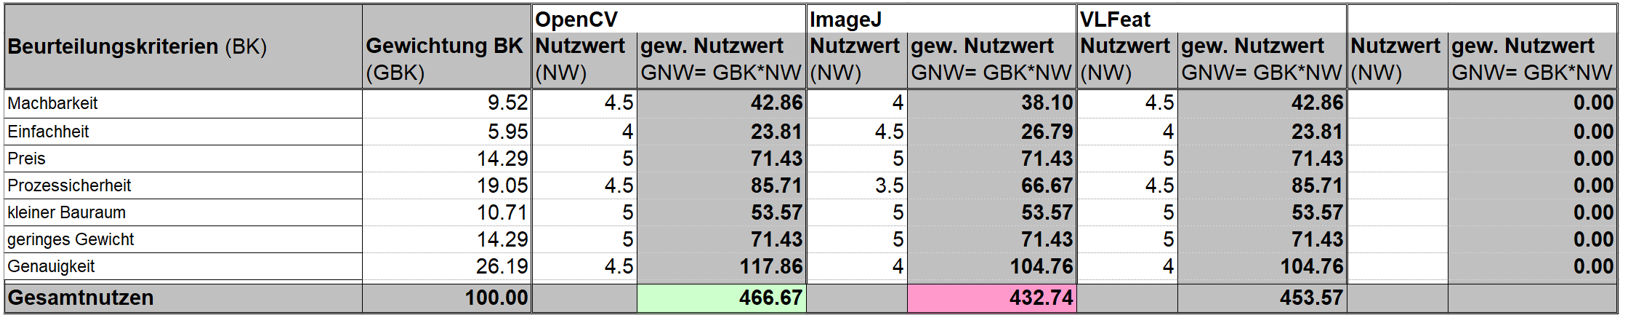
\includegraphics[width=1\textwidth]{Nutzwert_Vision.png}
            \caption{Nutzwertanalyse Vision Frameworks}
            \label{fig:vision_nutzwert}
        \end{figure}

        \vspace{0.5cm}
        \subsubsection{Klassifikation}
        Die eigentliche Intelligenz für die Objekterkennung findet in der Klassifikation statt. Diese findet wie in Abbildung \ref{fig:vision_ablauf} nach der Bildverarbeitung statt. Die Klassifikation findet anhand von Machine- Learning Algorithmen statt. Diese werden im Vorfeld mit bestimmten Modellen trainiert. Wie bei den Bildverarbeitungsframework gibt es auch bei den Machine- Learning Frameworks mittlerweile viele verschiedene. Hier werden drei verschiedene Frameworks angeschaut.\\
        \pagebreak


        \textbf{OpenCV}\\
        Das OpenCV Framework wurde schon im Abschnitt Bildverarbeitung schon vorgestellt. Der Vorteil von OpenCV ist, dass sowohl Bildverarbeitungsalgorithmen wie auch gängige Machine- Learning Algorithmen vorhanden sind. Diese gängigen ML- Algorithmen reichen für die Anforderungen aus.
        \begin{flushleft}
            \begin{table}[h]
            \begin{tabular}{ | l | p{11cm} |}
            \hline
            \textbf{Framework} & OpenCV \\ \hline
            \textbf{Programmiersprache} & C++, Java, Python \\ \hline
            \textbf{Betriebssystem} & plattformunabhängig \\ \hline
            \textbf{Lizenz} & BSD \\ \hline
            \textbf{Bewertung} &  \begin{itemize}
                                    \item[+] Performance
                                    \item[+] Konfigurationen
                                    \item[+] plattformunabhängig 
                                    \item[-] Lernkurve
                                  \end{itemize} \\ \hline
            \end{tabular}
            \caption{Konzeptbeurteilung: Machine- Learning Algorithmen OpenCV}
            \label{tab:konzept_ML_OpenCV}
            \end{table}
        \end{flushleft}
        \vspace{1cm}

        \textbf{Tensorflow}\\
        TensorFlow ist ein Framework zur datenstromorientierten Programmierung. Es wird aus Python-Programmen heraus benutzt und ist in Python und C++ implementiert. Populäre Anwendung findet TensorFlow im Bereich des maschinellen Lernens. In der Forschung und im Produktivbetrieb wird sie derzeit von verschiedenen Teams in kommerziellen Google-Produkten wie Spracherkennung, Gmail, Google Fotos und Google Suche verwendet.

        \begin{flushleft}
            \begin{table}[h]
            \begin{tabular}{ | l | p{11cm} |}
            \hline
            \textbf{Framework} & TensorFlow \\ \hline
            \textbf{Programmiersprache} & C++, Python \\ \hline
            \textbf{Betriebssystem} & plattformunabhängig \\ \hline
            \textbf{Lizenz} & Apache 2.0 open \\ \hline
            \textbf{Bewertung} &  \begin{itemize}
                                    \item[+] Performance
                                    \item[+] Community
                                    \item[+] plattformunabhängig 
                                    \item[-] Lernkurve
                                    \item[-] Komplexität 
                                  \end{itemize} \\ \hline
            \end{tabular}
            \caption{Konzeptbeurteilung: Machine- Learning Algorithmen Tensorflow}
            \label{tab:konzept_ML_Tensorflow}
            \end{table}
        \end{flushleft}
        \pagebreak

        \textbf{Caffe}\\
        Caffe ist eine Programmbibliothek für Deep Learning. Sie wurde von Yangqing Jia während seiner Ph.D.-Zeit am Vision and Learning Center der University of California, Berkeley entwickelt. Caffe hat zuerst die MATLAB-Implementierung von schnellen Convolutional Neural Networks (CNN) nach C und C++ portiert. Caffe enthält zahlreiche Algorithmen und Deep-Learning-Architekturen für die Klassifikation und Clusteranalyse von Bilddaten.
        

        \begin{flushleft}
            \begin{table}[h]
            \begin{tabular}{ | l | p{11cm} |}
            \hline
            \textbf{Framework} & Caffe \\ \hline
            \textbf{Programmiersprache} & C++ \\ \hline
            \textbf{Betriebssystem} & plattformunabhängig \\ \hline
            \textbf{Lizenz} & BSD \\ \hline
            \textbf{Bewertung} &  \begin{itemize}
                                    \item[+] Performance
                                    \item[+] plattformunabhängig 
                                    \item[-] Lernkurve
                                    \item[-] Komplexität 
                                    \item[-] Community 
                                  \end{itemize} \\ \hline
            \end{tabular}
            \caption{Konzeptbeurteilung: Machine- Learning Algorithmen Caffe}
            \label{tab:konzept_ML_Caffe}
            \end{table}
        \end{flushleft}

        \vspace{1cm}

        \textbf{Zusammenfassung Klassifikation: }
        Alle drei Frameworks verfügen über mächtige ML- Algorithmen und sind auch in ihrer Performance sehr ähnlich. Tensorflow verfügt über eine breite Community, welche in der Entwicklung von ML- Anwendungen helfen können. Doch der Vorteil, dass für die Bildverarbeitung so wie für die Klassifikation mit der gleichen Framework abdecken können, verhilft OpenCV auch im Bereich Klassifikation zum Gewinner. Alle benötigten ML- Algorithmen gibt es auch in OpenCV und so muss man sich nicht mit Konvertierungen und anderen Problematiken beim verwenden von mehreren Frameworks beschäftigen.


        \begin{figure}[H] 
            \centering
            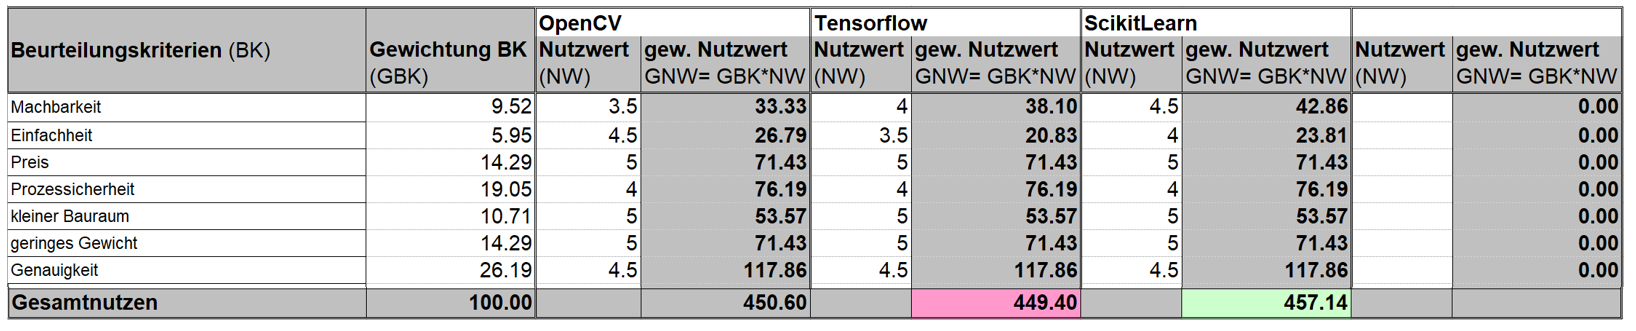
\includegraphics[width=1\textwidth]{Nutzwert_machineLearning.png}
            \caption{Nutzwertanalyse Klassifikation Frameworks}
            \label{fig:ML_nutzwert}
        \end{figure}



        
    
    
    
    
    \end{document}
